
\ifdefined\included
\else
\setcounter{chapter}{0} %% Numéro du chapitre précédent ;)
\dominitoc
\faketableofcontents
\fi

\chapter{Introduction}
\minitoc

\section{A prototypical scenario}

\section{Interacting with a robot: What can we expect ?}

\section[Knowledge organization]{Knowledge organization: Drawing inspiration from cognitive psychology }

Even if our goal in robotics is not to create a copy of the human, that it is in terms of body shape or cognition, taking inspiration from it is nether less important. In the same way that roboticists take inspiration from the human body to create robots able to evolve in a world created by and for the human, the field of cognitive robotic takes inspiration of the human cognition to create robots able to interact with humans. While we do not aim a making a copy of human cognition, we think that a robot must endow similar capabilities if we want them to interact with us acceptably and efficiently.

Regarding the knowledge representation, the first experimental study has been realized in 1885 by Ebbinghaus~\cite{ebbinghaus_1885_gedachtnis}. Since then, the definition of memory as the capacity to encode, store, and retrieve knowledge \cite{roediger_1996_retrieval} has been widely accepted. At the same time, the word "memory" has become a generic term suggesting a unique system. However, the human memory can rather be seen as several sub-systems that differ from their storage duration, storage capacity, and the level of consciousness necessary for information retrieval. In the rest of the section, we present some memory models, presented in a non-chronological way, and focussing on what is called long-term memory. During all this section, it is important to keep in mind that we only present models aiming to understand human cognition with a focus on knowledge management. No formal truth is stated here. The presented models and terms will allow us to better understand the existing robotic cognitive architectures and give inspiration for the design and structuration of the components developed during this thesis.

The primary division of the memory is done concerning the storage duration and capacity. From there has been defined the \textbf{short-term memory} (STM) and the \textbf{long-term memory} (LTM) \cite{atkinson_1966_some}. Short-term memory is characterized by its small capacity and its capability to retrieve information that has just been seen. We often hear about twenty seconds and seven items (or chunks). Long-term memory, on the opposite, refers to any situation where we use information that has not just be seen. We often hear about infinite capacity and duration. It is this latter that allows the acquisition of new knowledge and the retrieval of information acquired a long time ago.

Over the years, what was called short-term memory has become the \textbf{working memory} (WM) \cite{baddeley_1986_dementia}. This change has been made to add a notion of knowledge manipulation. Instead of focusing on the only temporal aspect, it reflects its functional aspect. It is thus a system that retains information for the time necessary for its use by other cognitive functions. The working memory and the long-term memories are two independent but related systems. For information to be stored in long-term memory, we think that it has to pass by the working memory.

For the structure of the long-term memory, a first dichotomy is proposed by Graf and Schacter \cite{graf_1985_implicit} with the \textbf{implicit} and \textbf{explicit} memory. It reflects the way knowledge can be retrieved. Knowledge from explicit memory can be retrieved consciously and voluntarily. On the opposite, knowledge from the implicit memory is retrieved in situations in which our comportments are influenced by an experience. This is the case when you pour water into a glass. We do not need to retrieve explicitly how to perform this task. It is our experience that influences how we do it.

Another dichotomy has been proposed by Squire and Cohen \cite{squire_1982_remote} with the \textbf{procedural} and \textbf{declarative} memory. Procedural memory is the system allowing us to retain knowledge about our cognitive, motor, or perceptual skills. It is the memory of the know-how. A particularity of this memory is that it is difficult to speak about the knowledge it stores and we use them unconsciously. The declarative memory stores representations of facts, events, general knowledge, and memories of past events. This knowledge can be retrieved consciously and we can speak about them. Taking the example of the code of your credit card. Initially, this knowledge is store in the declarative memory. When you need it you can easily remember it at say it. The more you use it and it slowly becomes an automatism. It became hard to remember it consciously while you use it every day and if you need to say it you can type it on a virtual keyboard to remember it. It has slowly moved into your procedural memory. We see that both dichotomies are almost equivalent. The declarative memory of Squire is related to the implicit memory of Graf, and the procedural one is related to the implicit memory.

Going deeper into the declarative memory, Tulving has proposed a dichotomy between \textbf{episodic} and \textbf{semantic} memory \cite{tulving_1995_organization}. The episodic memory retains knowledge related to past experienced events, which are specific to our individual experience, and localized both in space and time. The semantic memory is more general and retains knowledge that we accumulate all along with our life concerning our environment. It can be seen as an encyclopedic memory independent of the acquisition context. While the episodic memory is related to "remembering", the sematic one is related to "knowing". Taking as an example your visit to Toulouse \footnote{If you never visit it, you can take another city you have visited but you should plan to visit it anyway.}, this visit is encoded in the episodic memory while the knowledge that Toulouse is a city in France is encoded in the semantic one.

\begin{figure}[h!]
\centering
\includegraphics[scale=0.45]{figures/introduction/SPI.png}
\caption{\label{fig:SPI} Relations between episodic memory and semantic memory according to the SPI (Serial, Parallel, and Independent) model of Tulving (1995).}
\end{figure}

With the previous example, we saw that even if these two sub-systems of the declarative memory are independent, they are therefore in interaction with eachother as we can apply a semantic treatment on the episodic memory. To better undertand their relation, Tulving has proposed Serial, Parallel, and Independent model (SPI). As illustrated in Figure~\ref{fig:SPI}, the encoding of an information is serial (S) passing first by the semantic memory then in the episodic one. The storage in both memories is performed in parallel (P). Finally, the information recovery is independy between the two memories.
As we explain in the begin of this section, the presented theory can not be proven and must therefore be taken as~\cite{tulving_1995_organization} "an explicit starting point for a more systematic pursuit of what is clearly the next problem that needs to be tackled".

\section{Contributions}

\subsection{Knowledge representation}

\subsection{Knowledge exploitation}

\section{A reader's guide}


